
% Document class: article with font size 11pt
% ---------------
\documentclass[11pt,a4paper]{report}

% Call packages
% ---------------
\usepackage{comment} %Possible to comment larger sections
%http://get-software.net/macros/latex/contrib/comment/comment.pdf
\usepackage[T1]{fontenc} %oriented to output, that is, what fonts to use for printing characters.
\usepackage[utf8]{inputenc} %allows the user to input accented characters directly from the keyboard
%Put fontenc before inputenc
\usepackage{fourier} %Better typeface
%http://mirrors.dotsrc.org/ctan/fonts/fourier-GUT/doc/latex/fourier/fourier-doc-en.pdf
\usepackage[danish]{babel}														     % Danish
\usepackage[protrusion=true,expansion=true]{microtype}				                 % Better typography
%http://www.khirevich.com/latex/microtype/
\usepackage{amsmath,amsfonts,amsthm, amssymb}							 % Math packages
\usepackage[pdftex]{graphicx} %puts to pdf and graphic
%http://www.kwasan.kyoto-u.ac.jp/solarb6/usinggraphicx.pdf
\usepackage{xcolor,colortbl}
%http://mirrors.dotsrc.org/ctan/macros/latex/contrib/xcolor/xcolor.pdf
%http://texdoc.net/texmf-dist/doc/latex/colortbl/colortbl.pdf
\usepackage{tikz} %documentation http://www.ctan.org/pkg/pgf
\usepackage{parskip} %http://www.ctan.org/pkg/parskip
%http://tex.stackexchange.com/questions/51722/how-to-properly-code-a-tex-file-or-at-least-avoid-badness-10000
%Never use \\ but instead press "enter" twice. See second website for more info
\usepackage{natbib}
%\usepackage{tablefootnote}
%Brug H for figur lige HER!!
\usepackage{float}
%\caption{} til tabeller
\usepackage{caption}

\usepackage{pbox}

%Skal ikke bruges i slut
\usepackage[draft,danish]{fixme} %Danish latex book
%\usepackage{showkeys} %Brug kun til at holde styr på labels

%%--------------------------------
%Til at vise links i pdf filen så man kan hoppe frem og tilbage
\usepackage{hyperref}
\hypersetup{
    colorlinks,
    linkcolor={blue!35!black},
    citecolor={blue!50!black},
    urlcolor={blue!80!black}
}

\usepackage{fancyhdr} % Required for custom headers
\usepackage{lastpage} % Required to determine the last page for the footer
\usepackage{extramarks} % Required for headers and footers
\usepackage{listings} % Required for insertion of code
\usepackage{courier} % Required for the courier font
\usepackage{lipsum} % Used for inserting dummy 'Lorem ipsum' text into the template


\usepackage[top=1in, bottom=1.25in, left=1.25in, right=1.25in, footskip=0.25in]{geometry}

\linespread{1.15} % Line spacing

% Set up the header and footer
\pagestyle{fancy}
\lhead{\hmwkAuthorName} % Top left header
\chead{\hmwkClass\: \hmwkTitle} % Top center head
\rhead{\firstxmark} % Top right header
\lfoot{\lastxmark} % Bottom left footer
\cfoot{} % Bottom center footer
\rfoot{Page\ \thepage\ of\ \protect\pageref{LastPage}} % Bottom right footer
\renewcommand\headrulewidth{0.4pt} % Size of the header rule
\renewcommand\footrulewidth{0.4pt} % Size of the footer rule

\setlength\parindent{0pt} % Removes all indentation from paragraphs

%----------------------------------------------------------------------------------------
%	DOCUMENT STRUCTURE COMMANDS
%	Skip this unless you know what you're doing
%----------------------------------------------------------------------------------------

% Header and footer for when a page split occurs within a problem environment
\newcommand{\enterProblemHeader}[1]{
\nobreak\extramarks{#1}{#1 continued on next page\ldots}\nobreak
\nobreak\extramarks{#1 (continued)}{#1 continued on next page\ldots}\nobreak
}

% Header and footer for when a page split occurs between problem environments
\newcommand{\exitProblemHeader}[1]{
\nobreak\extramarks{#1 (continued)}{#1 continued on next page\ldots}\nobreak
\nobreak\extramarks{#1}{}\nobreak
}

\setcounter{secnumdepth}{0} % Removes default section numbers
\newcounter{homeworkProblemCounter} % Creates a counter to keep track of the number of problems

\newcommand{\homeworkProblemName}{}
\newenvironment{homeworkProblem}[1][Task \arabic{homeworkProblemCounter}]{ % Makes a new environment called homeworkProblem which takes 1 argument (custom name) but the default is "Problem #"
\stepcounter{homeworkProblemCounter} % Increase counter for number of problems
\renewcommand{\homeworkProblemName}{#1} % Assign \homeworkProblemName the name of the problem
\section{\homeworkProblemName} % Make a section in the document with the custom problem count
\enterProblemHeader{\homeworkProblemName} % Header and footer within the environment
}{
\exitProblemHeader{\homeworkProblemName} % Header and footer after the environment
}

\newcommand{\problemAnswer}[1]{ % Defines the problem answer command with the content as the only argument
\noindent\framebox[\columnwidth][c]{\begin{minipage}{0.98\columnwidth}#1\end{minipage}} % Makes the box around the problem answer and puts the content inside
}

\newcommand{\homeworkSectionName}{}
\newenvironment{homeworkSection}[1]{ % New environment for sections within homework problems, takes 1 argument - the name of the section
\renewcommand{\homeworkSectionName}{#1} % Assign \homeworkSectionName to the name of the section from the environment argument
\subsection{\homeworkSectionName} % Make a subsection with the custom name of the subsection
\enterProblemHeader{\homeworkProblemName\ [\homeworkSectionName]} % Header and footer within the environment
}{
\enterProblemHeader{\homeworkProblemName} % Header and footer after the environment
}

%----------------------------------------------------------------------------------------
%	NAME AND CLASS SECTION
%----------------------------------------------------------------------------------------

\newcommand{\hmwkTitle}{Assignment\ \#2} % Assignment title
\newcommand{\hmwkDueDate}{Sunday,\ November\ 29,\ 2015} % Due date
\newcommand{\hmwkClass}{Compilers} % Course/class
\newcommand{\hmwkClassTime}{Task 1, 2} % Class/lecture time
\newcommand{\hmwkClassInstructor}{Resubmit:} % Teacher/lecturer
\newcommand{\hmwkAuthorName}{Mirza Hasanbasic} % Your name

%----------------------------------------------------------------------------------------
%	TITLE PAGE
%----------------------------------------------------------------------------------------

\title{
\vspace{2in}
\textmd{\textbf{\hmwkClass:\ \hmwkTitle}}\\
\normalsize\vspace{0.1in}\small{Due\ on\ \hmwkDueDate}\\
\vspace{0.1in}\large{\textit{\hmwkClassInstructor\ \hmwkClassTime}}
\vspace{3in}
}

\author{\textbf{\hmwkAuthorName}}
\date{} % Insert date here if you want it to appear below your name


%----------------------------------------------------------------------------------------
%	MATH
%----------------------------------------------------------------------------------------
%\newcommand{\Real}{\mathbb R}
%\newcommand{\Complex}{\mathbb C}
%\newcommand{\Field}{\mathbb F}
%\newcommand{\RPlus}{[0,\infty)}
%%
%\newcommand{\norm}[1]{\left\Vert#1\right\Vert}
%\newcommand{\essnorm}[1]{\norm{#1}_{\text{\rm\normalshape ess}}}
%\newcommand{\abs}[1]{\left\vert#1\right\vert}
%\newcommand{\set}[1]{\left\{#1\right\}}
%\newcommand{\seq}[1]{\left<#1\right>}
%\newcommand{\eps}{\varepsilon}
%\newcommand{\To}{\longrightarrow}
%\newcommand{\RE}{\operatorname{Re}}
%\newcommand{\IM}{\operatorname{Im}}
%\newcommand{\Poly}{{\cal{P}}(E)}
%\newcommand{\EssD}{{\cal{D}}}
%% THEOREMS ----------------------------------------------------------------
%\theoremstyle{plain}
%\newtheorem{thm}{Theorem}[section]
%\newtheorem{cor}[thm]{Corollary}
%\newtheorem{lem}[thm]{Lemma}
%\newtheorem{prop}[thm]{Proposition}
%%
%\theoremstyle{definition}
%\newtheorem{defn}{Definition}[section]
%%
%\theoremstyle{remark}
%\newtheorem{rem}{Remark}[section]
%%
%\numberwithin{equation}{section}
%\renewcommand{\theequation}{\thesection.\arabic{equation}}


\lstset{
  frame=single,
  numbers=left,
  mathescape,
  literate={->}{$\rightarrow$}{2}
           {ε}{$\varepsilon$}{1}
           {=>}{$\Rightarrow$}{2}
}

\begin{document}

\maketitle

%----------------------------------------------------------------------------------------
%	TABLE OF CONTENTS
%----------------------------------------------------------------------------------------

%\setcounter{tocdepth}{1} % Uncomment this line if you don't want subsections listed in the ToC

\newpage
\tableofcontents
\newpage

%----------------------------------------------------------------------------------------
%	PROBLEM 1
%----------------------------------------------------------------------------------------

% To have just one problem per page, simply put a \clearpage after each problem


\begin{homeworkProblem}
\textbf{a)}

\[
([og][og])^*|([og][og][og])^*
\]

Her vil vi have et alfabet, hvor sekvensen af længden er delelig med 2 eller 3.

\textbf{b)}

\begin{align*}
  T \rightarrow& c \\
  R \rightarrow& c T \\
  T \rightarrow& a T b \\
\end{align*}

Vil producerer en context-free grammer, hvor c er tilladt til at være alene, c vil altid være mellem a og b og der vil, for hvert a være et b.

\textbf{c)}

\textbf{i)}

Når man har \emph{\% prec letprec}, så specificerer det en regel, som er associativ med \emph{letprec} i dette tilfælde. I \emph{\% nonassoc} har man indikeret at \emph{letprec} ikke er associativ, altså vores \emph{LET} og \emph{IN}.

\textbf{ii)}

\textcolor[rgb]{0.76,0.00,0.02}{\textbf{FIX:}}

Det som \emph{let} gør, er at, der gives et eller flere udtryk, som deklareres en værdi, hvor disse værdier så udgør et resultet til sidst.

Hvor den første variabel består af en streng, et udtryk og så positionen af angivelsen.
Altså, hvis så kigger, på \texttt{(Dec (\#1 \$2, \$4, \$3), \$6, \$1)}, så har vi, at \#1 \$2 vil refere til den første parameter og andet symbol, ID, som er en streng der holder navnene på variablene.

\$4 vil så refere til parameteren af det fjerde i udtrykket som det vil blive båndet til. Hvor \$3 så er symbolet EQ, da det er på denne position, og dermed vil det være til et lighedstegn, som den vil blive båndet til.

For at kigge på de sidste to, kigger vi på hele udtrykket, altså \texttt{Let (Dec (\#1 \$2, \$4, \$3), \$6, \$1)}. Her har vi at \$6 referer til hvilken erklæring af variablen, (Dec) vil blive brugt og hvor \$1 referer til positionen af let symbolet

\end{homeworkProblem}

\begin{homeworkProblem}

\textbf{a)}

For filter, vil det altså være

\[
\forall\alpha \quad  ((\alpha\rightarrow\texttt{bool})*[\alpha])\rightarrow [\alpha]
\]

\textcolor[rgb]{0.76,0.00,0.02}{\textbf{FIX:}}

\textbf{b)}

\begin{lstlisting}
Check$_{Exp}$(Exp, vtable, ftable) = case Exp of

    filter(p, arr_exp) =>
        t$_{arr}$ = Check$_{Exp}$(arr$_{exp}$), vtable, ftable)
        t$_{el}$ = case t$_{arr}$ of
                   Array(t$_1$) -> t$_1$
                |  other -> error()

        t$_{f}$ = lookup(ftable, name(p))
        case t$_{f}$ of
             (t$_{in}$ -> t$_{out}$) => if t$_{in}$ = t$_{el}$ and t$_{out}$ = bool
                                        then t$_{arr}$
                                        else error()
           | _ => error()
\end{lstlisting}

\textbf{c)}

\begin{lstlisting}
Check$_{Exp}$(Exp, vtable, ftable) = case Exp of

    filter( Lambda(ret_type, id_type_lst, body), arr_exp) =>
        t$_{body}$ = Check$_{Exp}$(body, vtable, ftable)
        t$_{arr}$ = Check$_{Exp}$(arr$_{exp}$), vtable, ftable)
        t$_{el}$ = case t$_{arr}$ of
                   Array(t$_1$) -> t$_1$
                |  other -> error()
        t$_{in}$ = case id_type_lst of
                   [(_,t$_2$)] -> t$_2$
                |  other -> error()
        if ret_type = bool and t$_{body}$ = bool and t$_{el}$ = t$_{in}$
        then t$_{arr}$
        else error()
\end{lstlisting}

\end{homeworkProblem}

\begin{homeworkProblem}
Figuren under er et eksempel på hvordan man kan bruge MGU algoritmen 

\begin{figure}[H]
  \centering
  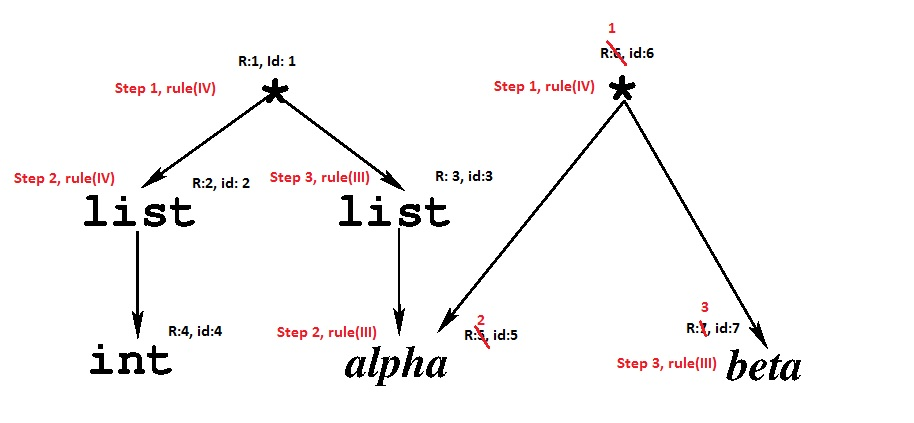
\includegraphics[scale=0.7]{MGU.jpg}
\end{figure}

list(int) * list(list(int))



\end{homeworkProblem}


\end{document} 